
\begin{figure}[t]
\centering
\ovalbox{
  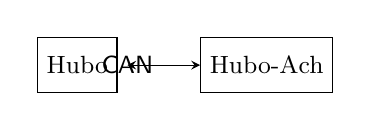
\begin{tikzpicture}
  \tikzstyle{cell} = [rectangle,minimum height=2.0em,minimum
  width=2.00em, font=\small,draw=black]
  \tikzstyle{vcell} = [rectangle,minimum height=2.0em,minimum
  width=2.00em, font=\small,draw=white]

  \tikzstyle{ref} =[->, >=stealth,out=0,in=-180]
  \tikzstyle{ref2} =[<->, >=stealth,out=0,in=-180]
%  \tikzstyle{ref} =[->, >=stealth,out=-90,in=90]

\node [matrix,nodes=draw] (hubo)
  {
    \node[cell,name=datfree]{Hubo};\\
  };
% \node [matrix,right of=hubo,xshift=2.0em] (index)
 \node [matrix,right of=hubo,xshift=4.0em] (index)
  {
    \node[cell,name=i3,font=\small]{Hubo-Ach}; \\
  };

 


%\node[name=hlabel,left of=header,xshift=-8em] {header};
%  \node[name=ilabel,left of=index,xshift=-8em] {index\_array};
%  \node[name=dlabel,left of=data,xshift=-8em] {data\_array};

%\path (hubo.east) edge[ref,out=-90,in=90] (i3.north);
\path [every node/.style={font=\sffamily\small}] 
      (hubo.east) edge[ref2,out=0,in=-180] (i3.west) node {CAN};

  \end{tikzpicture}

}


\end{figure}











